%!TEX root = paper.tex
%%%%%%%%%%%%%%%%%%%%%%%%%%%%%%%%%%%%%%%%%%%%%%%%%%%%%%%%%%%%%%%%%%%%%%%%%%%%%%%%
\section{Lag Simulation}
\label{sec:simulation}

Based on the introduced model a stochastic \textsc{Gnu R}-based \gls{DES} was created~\cite{onlinegame-lag-sim-repo} and several distinct game scenarios investigated. Due to the influence of several stochastic processes (user inputs $U$, network delay $D$, server processing time $P$) and the differing offset of the clocked processes, a sufficient number of repetitions is required to provide meaningful results. The investigations here are intended to highlight some particular aspect in each of the scenarios. First, the input is modeled by an exponential distribution with a rate of $20$ events per second. The offsets between the clocked processes are uniformly distributed in their respective intervals. It is further assumed that the server processing time $P$ follows a left-truncated normal distribution with $\mu_P = \SI{3}{\milli\second}$ and $\sigma_P = \SI{0.1}{\milli\second}$. Additionally, the rate $c$ at which command messages are sent to the game server is set equal to the server's tickrate $g$ as the server would not process more commands either way. This might however increase the \gls{E2E} lag in some situations if a command message just misses one of the server's ticks and has to wait another full cycle. The evaluation of the presented scenarios was conducted on the basis of $\np{1000}$ repetitions for each setting. Each run consisted of a series of $\np{100}$ input events and their associated \gls{E2E} lag values. On this basis a median lag was calculated.
% over the $n$ input events for each run $i$, and finally an overall mean lag out of the individual medians of each repetition, i.e. $\overline{T}=\frac{1}{n}\sum_{i=1}^r\widetilde{T_i}$.


%%%%%%%%%%%%%%%%%%%%%%%%%%%%%%%%%%%%%%%%%%%%%%%%%%%%%%%%%%%%%%%%%%%%%%%%%%%%%%%%
\subsection{Best Case Scenario: Local Game}
\label{subsec:local-game}

\begin{figure}[!t]
	\centering
	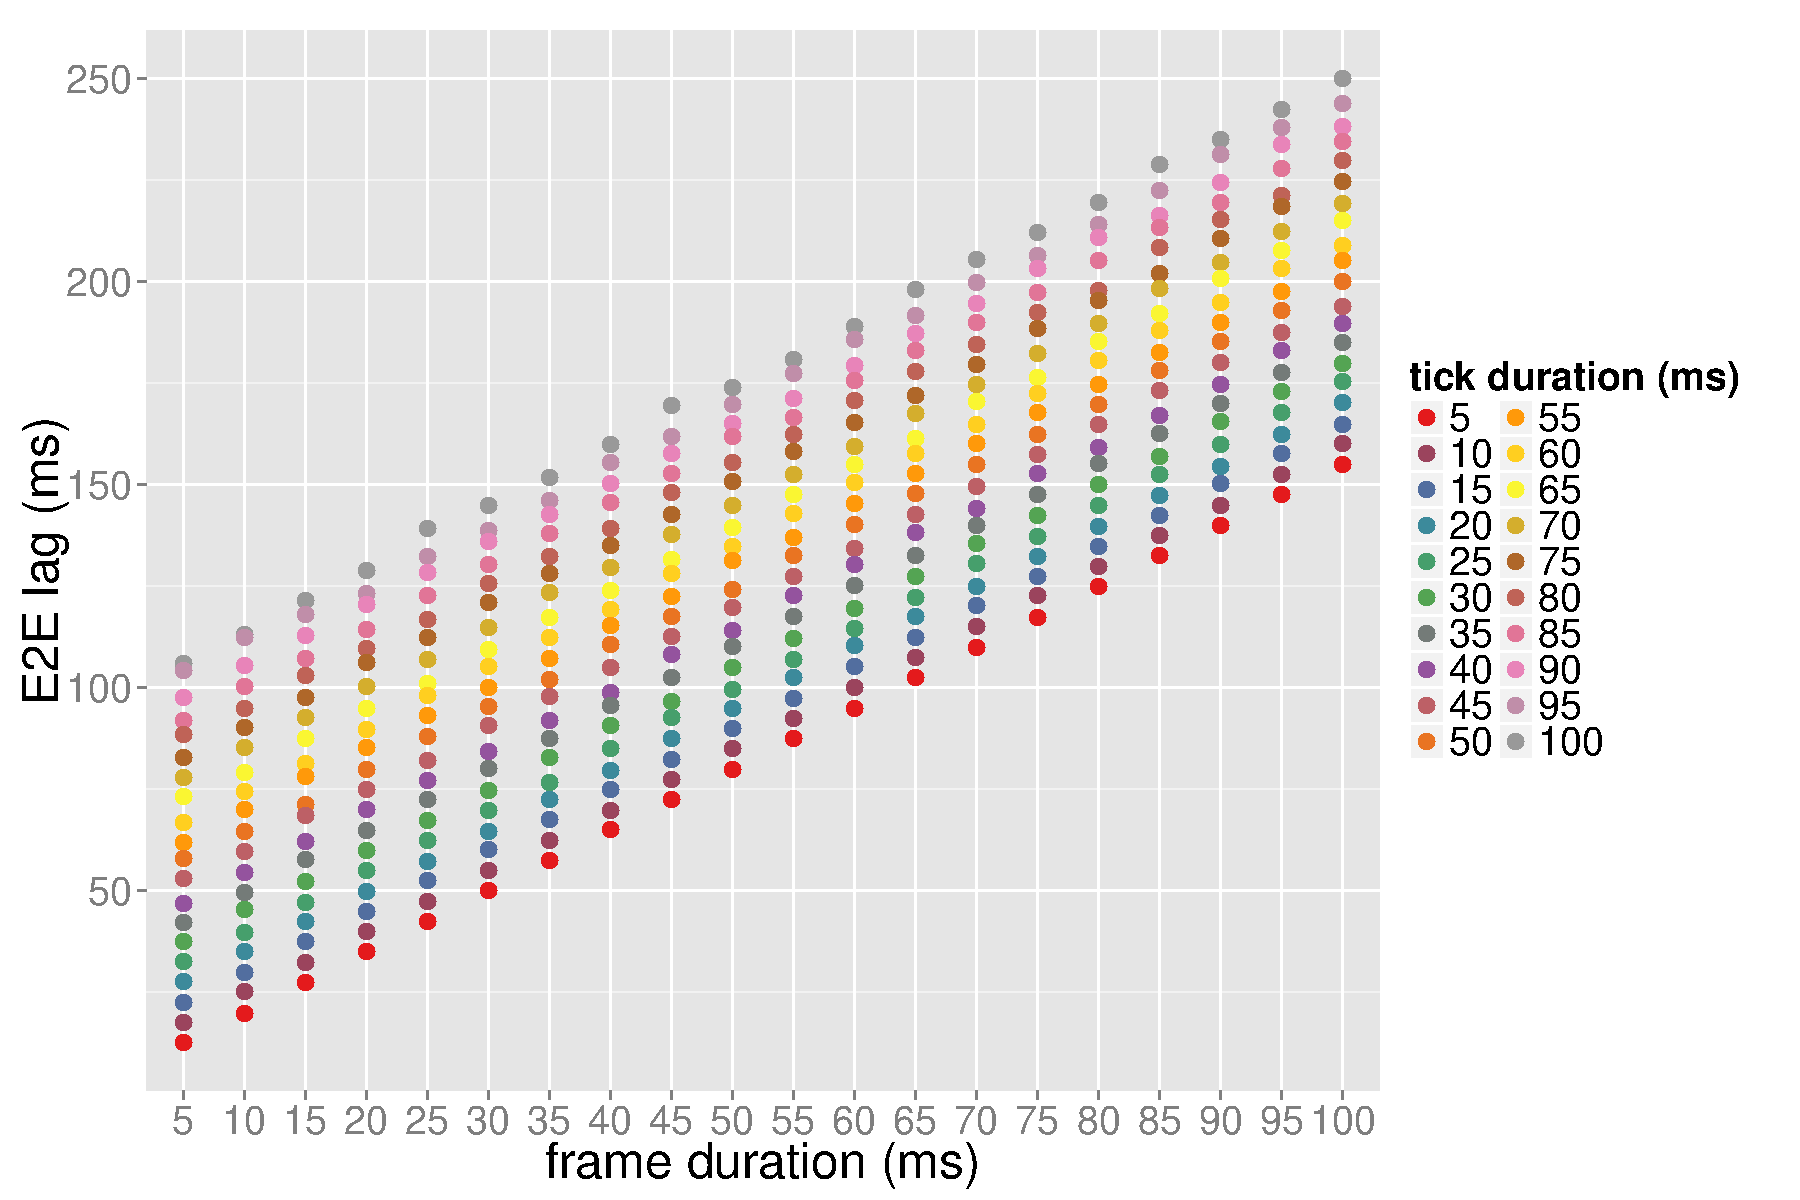
\includegraphics[width=1.0\columnwidth]{../../../simulation/visualization/nwless-onlinegame-1000rounds.pdf}
	\caption{Median \gls{E2E} lag under various frame and tick durations for a locally-running game (§\ref{subsec:local-game}). Lower lag values are achieved at lower frame and tick durations; the frame duration has a larger influence on the \gls{E2E} lag.}
\label{fig:nwless-scatter}
\end{figure}

The first and simplest scenario to be investigated here is the case of the local game. In the version implemented here, the tickrate at a locally running quasi-server component is still present, therefore representing the best case an online multiplayer game could achieve without any network influences. Figure~\ref{fig:nwless-scatter} plots the relationship between the frame duration (i.e., the inverse of the framerate), the tick duration, and the resulting median \gls{E2E} lag. Every user input event traverses three queues with fixed-rate outputs ($c=g$, $g$, and $f$). In the ideal case, an input event occurs just before the command queue cycles, correctly aligned with the following server tick and frame render cycles. In this case the \gls{E2E} lag will be slightly above the frame time that must elapse before the update can be rendered to screen, $T_{min}>f^{-1}$. In case the events are unfavorably offset against one another, an input event has to wait almost a full input cycle until it is processed further, reaching the server just after a tick has occurred, so it waits almost a full server tick. Ultimately, it has to wait for almost two frames until it is displayed.

Combined with the previous result the lag is bounded as follows, $f^{-1} < T < c^{-1}+g^{-1}+2f^{-1}$. The mid-interval point between these two limits is $T_{mid}=\frac{3}{2} f^{-1} + g^{-1}|_{c=g}$ which coincides roughly with the medians of the stochastic simulation. Looking at a typical \SI{60}{\hertz} video game with an equal tickrate (i.e. a frame duration of $\approx \SI{16.6}{\milli\second}$) the median lag is in the range of \SIrange{45}{50}{\milli\second}. So even under quasi-optimal circumstances and without factoring in the delay of the network and screen and input devices, there is already a considerable amount of \gls{E2E} lag. The expression for $T_{mid}$ and the simulation results also indicate that video games (and quality assessments thereof) should try to achieve the highest framerate possible to minimize its influence on the \gls{E2E} lag and thus \gls{QoE}.

%%%%%%%%%%%%%%%%%%%%%%%%%%%%%%%%%%%%%%%%%%%%%%%%%%%%%%%%%%%%%%%%%%%%%%%%%%%%%%%%
\subsection{Online Gaming}
\label{subsec:online-gaming}


\begin{figure}[!t]
	\centering
	\vspace{-6mm}
	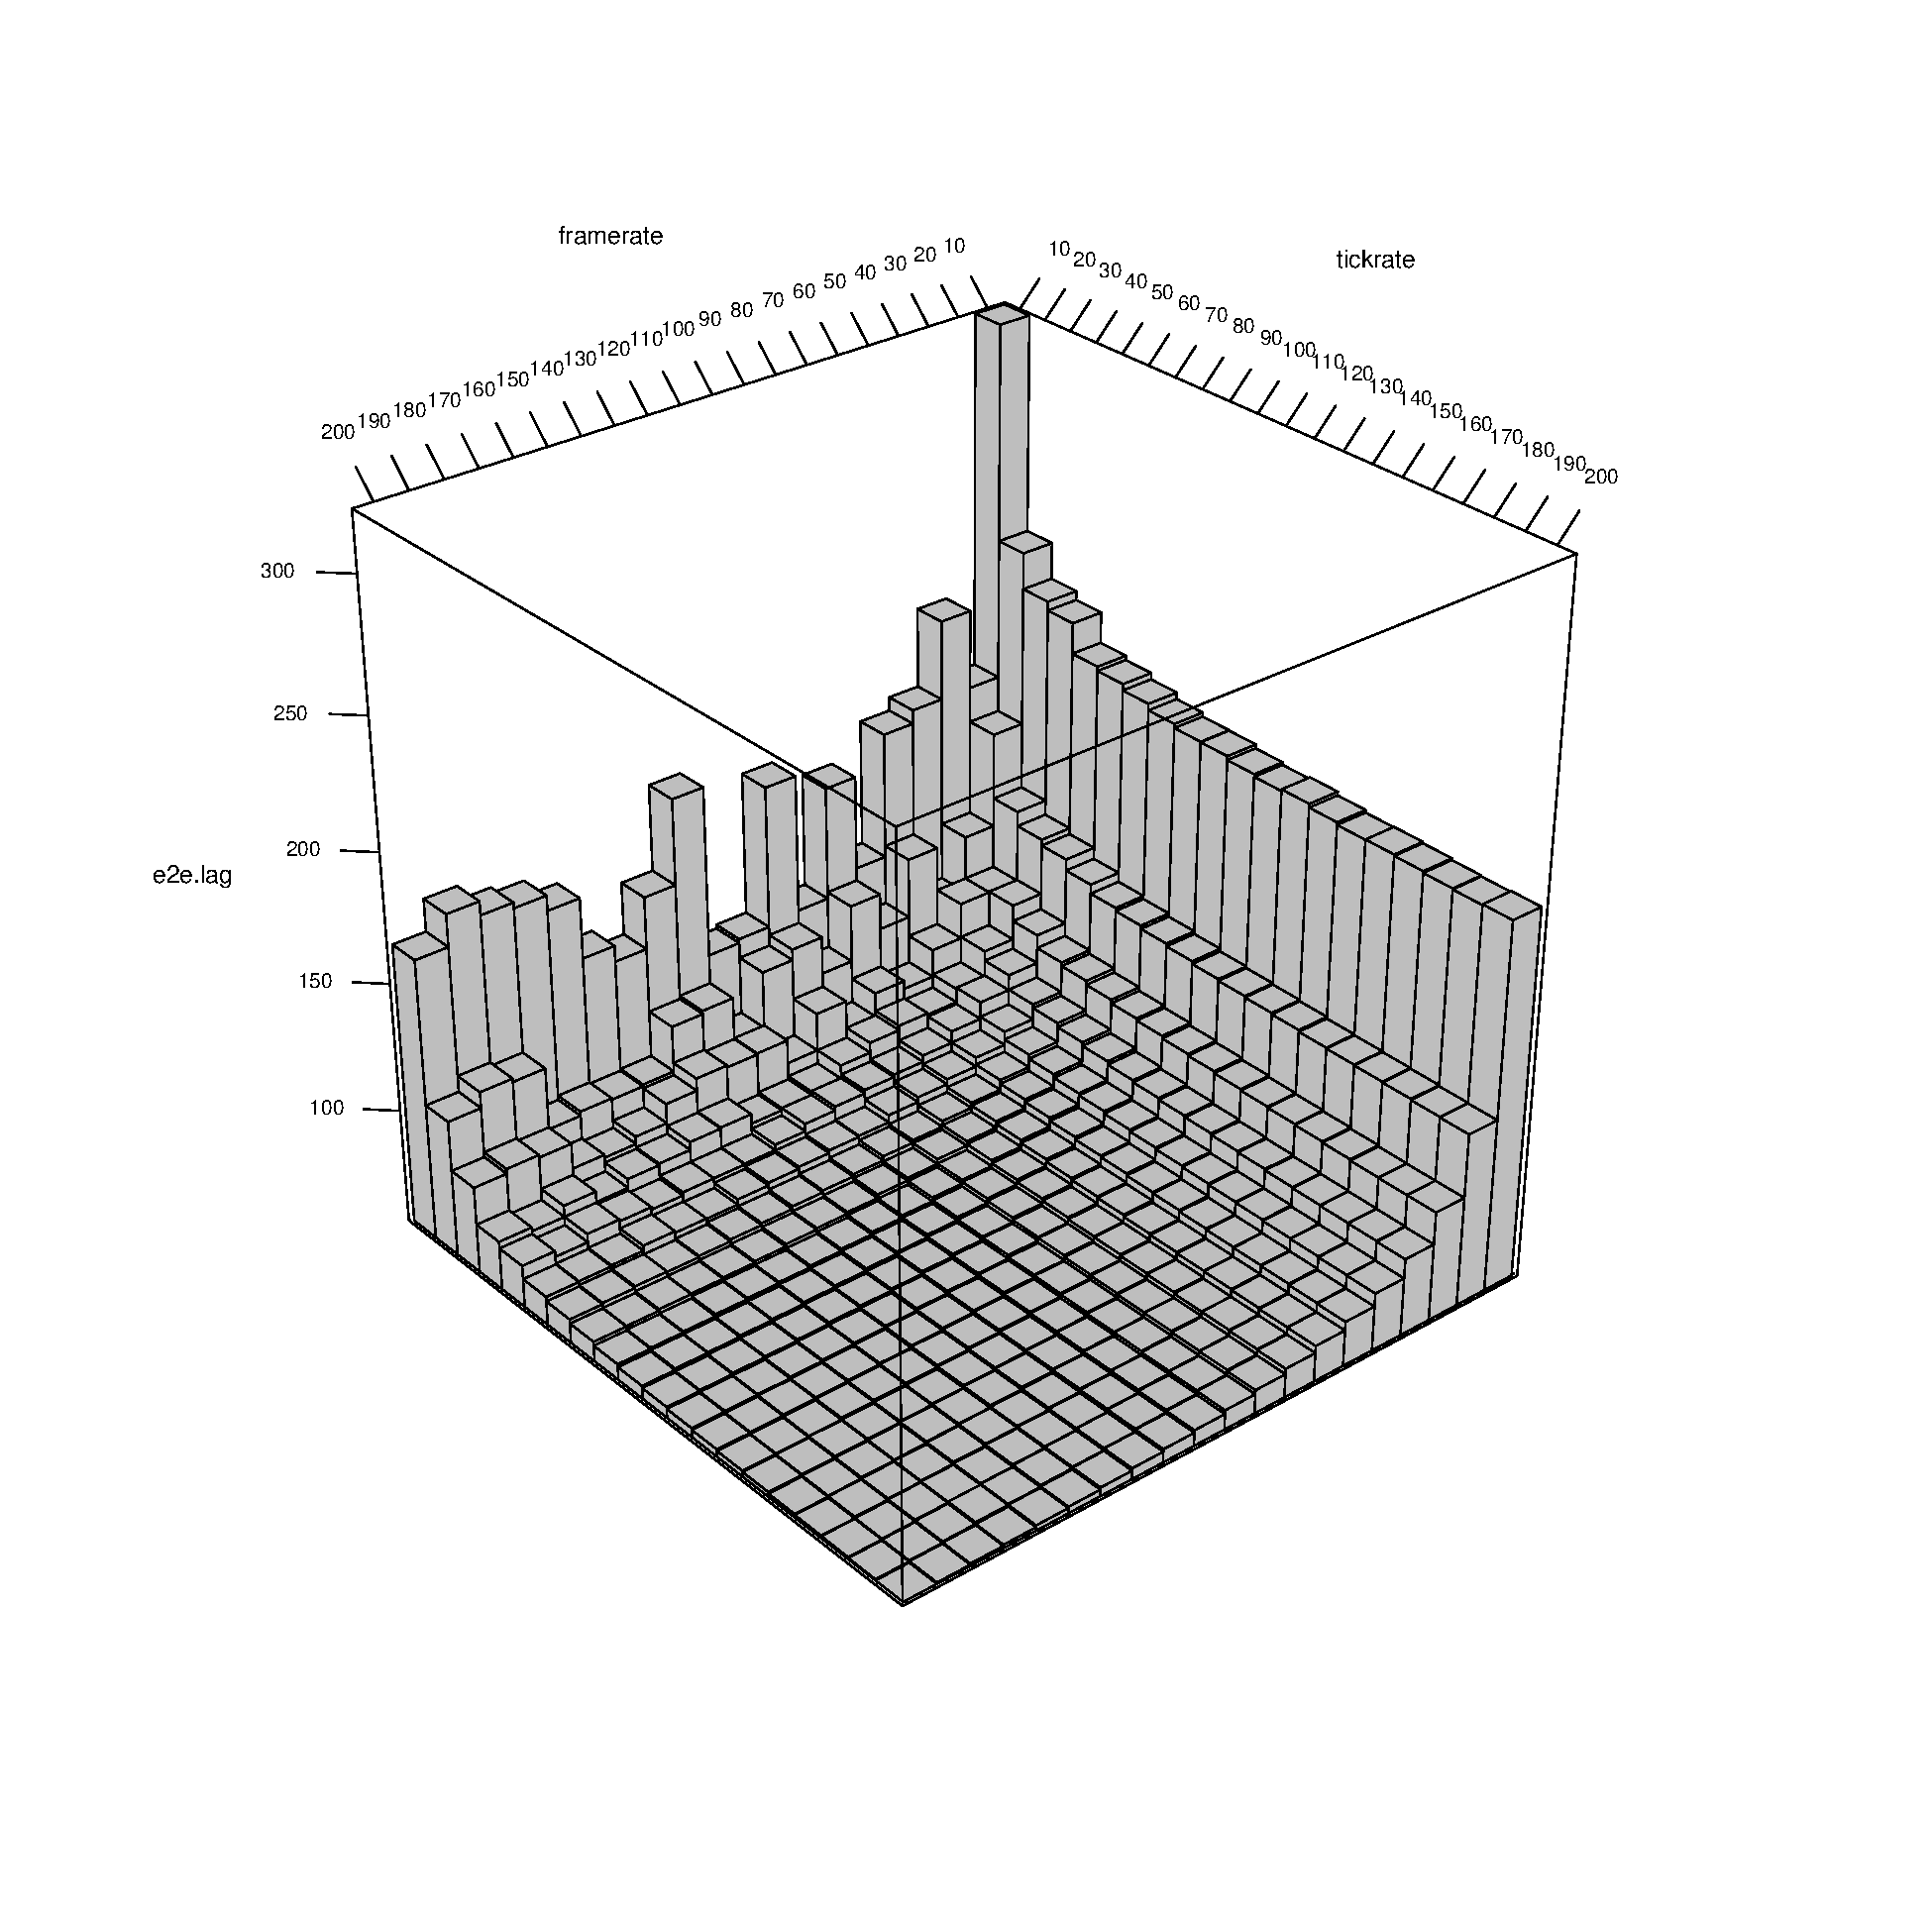
\includegraphics[width=1.0\columnwidth]{../../../simulation/visualization/e2e-lag-3dbars.pdf}
	\vspace{-15mm}
	\caption{Influence of client framerate and server tickrate on the median \gls{E2E} lag in the online game scenario (§\ref{subsec:online-gaming}). Only for high rates $f$, $g$, the lag is dominated by the network round-trip and server processing time, $T\approx2\mu_D+\mu_P=\SI{43}{\milli\second}$.}
\label{fig:3dbars-framerate-tickrate-lag}
\end{figure}

Next up is a more realistic online video game scenario, now with added network delay $D$ and server processing time $P$. For this exemplary scenario, the one-way delay $D$ was assumed to follow a left-truncated normal distribution, with $\mu_D = \SI{20}{\milli\second}$ and $\sigma_D = \SI{5}{\milli\second}$. Typical competitive online games today are expected to operate in such ranges. An \acrshort{RTT} of \SI{100}{\milli\second} is often considered to be the upper limit for a good playing experience. Two things can be noted of the influence of frame and tickrates in this scenario, see Fig.~\ref{fig:3dbars-framerate-tickrate-lag}. First, the framerate again has a larger influence on the lag than the tickrate. The reasoning follows from §\ref{subsec:local-game} above. Second, for low framerates and tickrates, the impact of network delay on the \gls{E2E} lag is almost completely masked. Only if both rates are high enough, the network delay will play a more significant role. This masking effect has large implications for video games and their evaluation. Many evaluations solely examine the influence of the network delay, without any consideration to other contributing factors. Our results indicate that this might not be the best course of action. The masking effect likely shifts to lower values of the frame- and tickrates when a higher network delay is examined.

%Another interesting result (not plotted here) is the much larger variance of lag in the framerate dimension when compared to the tickrate. This requires video game studies to have a very high repetition rate to provide meaningful results.


%%%%%%%%%%%%%%%%%%%%%%%%%%%%%%%%%%%%%%%%%%%%%%%%%%%%%%%%%%%%%%%%%%%%%%%%%%%%%%%%
\subsection{Cloud Gaming}
\label{subsec:cloud-gaming}

\begin{figure}[!t]
	\centering
	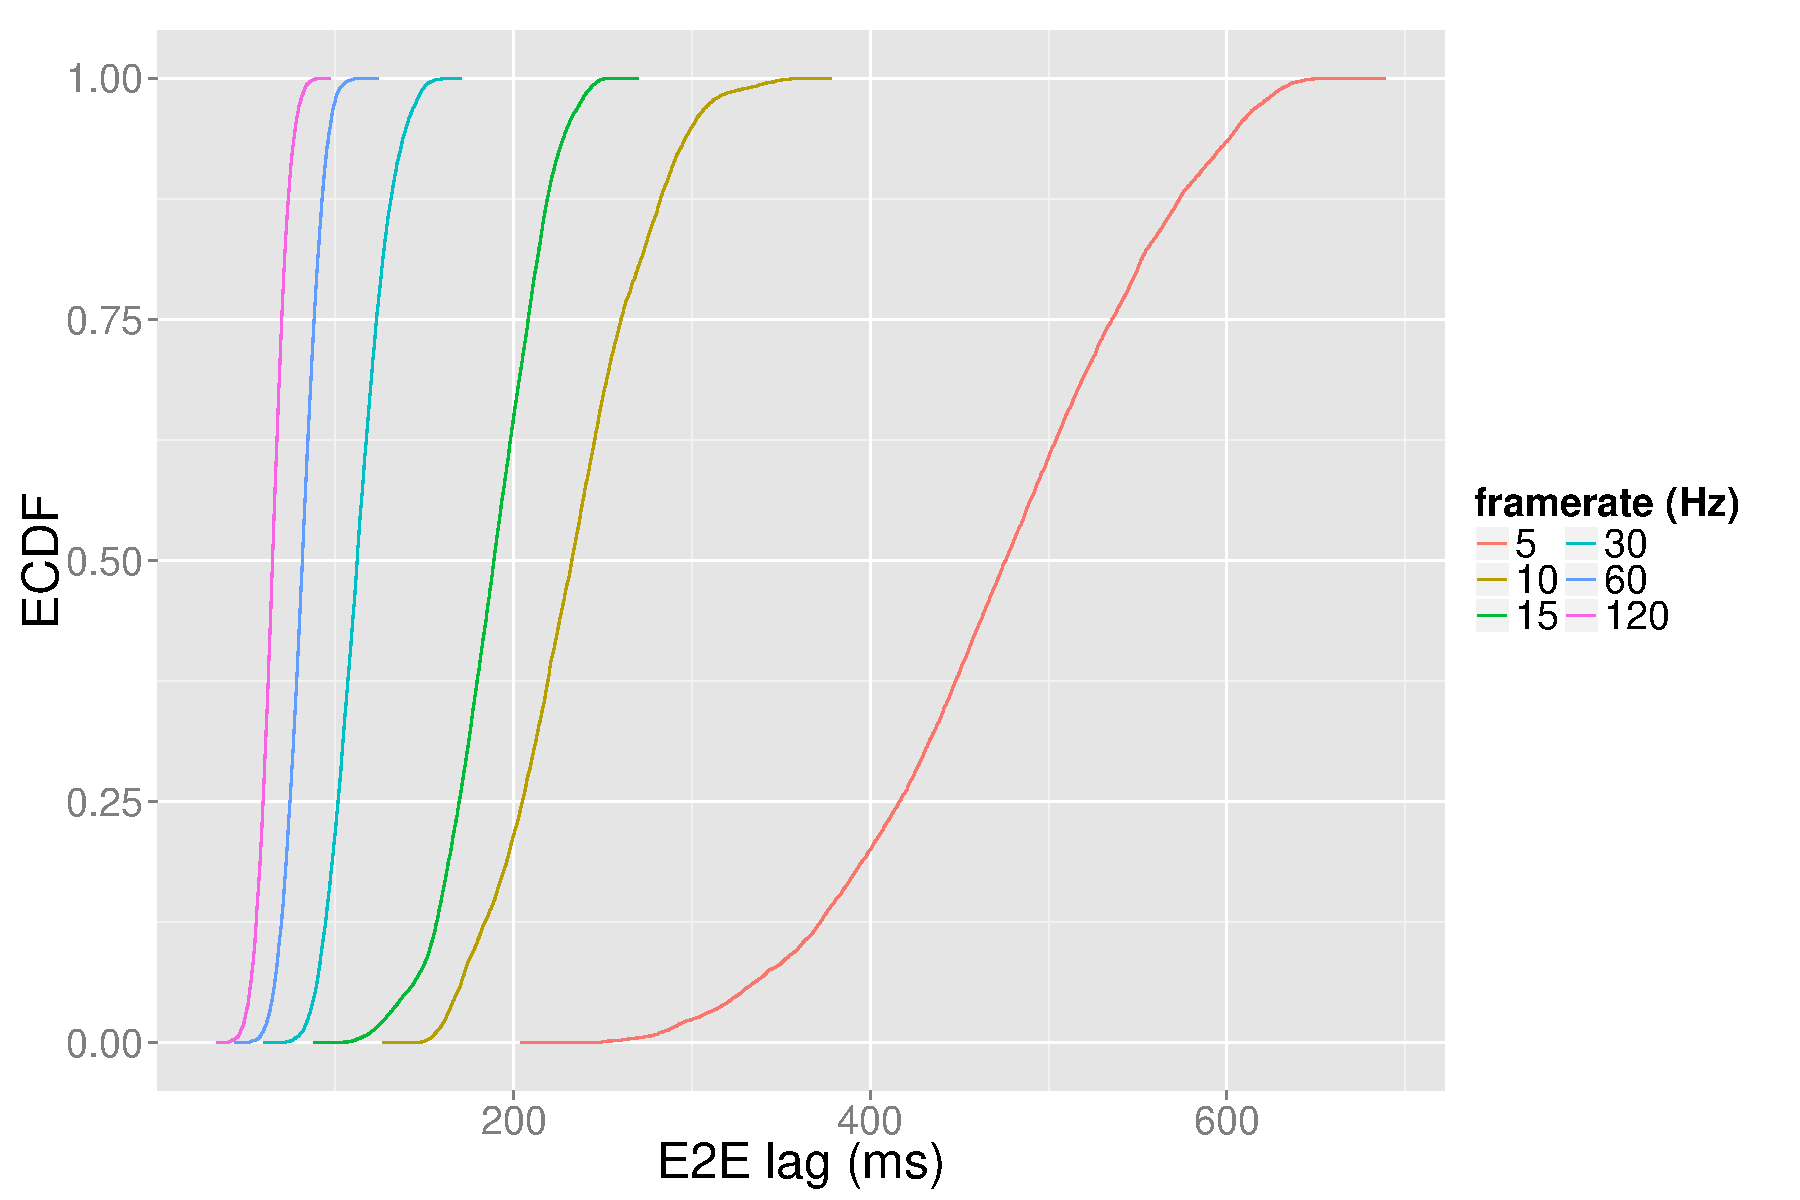
\includegraphics[width=1.0\columnwidth]{../../../simulation/visualization/cloudgaming-lag-cdf.pdf}
	\caption{Influence of the rendering and streaming framerate on the \gls{E2E} lag in the cloud scenario (§\ref{subsec:cloud-gaming}). The vertical reference line denotes the average server processing time, network round-trip and codec delay $\mu_P+2\mu_D+e+d=\SI{68}{\milli\second}$.}
\label{fig:cloud-e2e-delay-sim}
\end{figure}

The final simulation effort encompasses a cloud gaming scenario. Constant encode  and decode delays $e,d$ are in place at the game streaming server and client respectively. The frames are now generated by the server and need to be transported back to the client first. This is emulated by adding one frame time to account for the transmission of the encoded screen contents. Otherwise, the network model is kept as before. The command rate $c$ is set to $\SI{200}{\hertz}$. Figure~\ref{fig:cloud-e2e-delay-sim} shows the results of this scenario as \acrshort{ECDF}s of the \gls{E2E} lag for several framerates. As before, the framerate impacts the \gls{E2E} lag more severely than the network delay does. This result is of particular interest, considering how past studies have relied on similarly low framerates as $5-\SI{15}{\hertz}$ when assessing the network influence on cloud gaming \gls{QoE}. Similarly, these results can provide guidelines for implementors of cloud gaming to factor in the framerate in their calculations accordingly.


